\documentclass[a4paper]{article}
\usepackage[spanish]{babel}
\title{Taller 1}

\usepackage[utf8]{inputenc}
\usepackage{caratula}
\usepackage{graphicx}
\usepackage{color}
\usepackage{listings}
\usepackage{float}


\setlength{\leftmargin}{2cm}
\setlength{\rightmargin}{2cm}
\setlength{\oddsidemargin}{-1cm}
\setlength{\evensidemargin}{-1cm}
\setlength{\topmargin}{-1cm}
\setlength{\textwidth}{18cm}
\setlength{\textheight}{25cm}

\usepackage{fancyhdr}
\pagestyle{fancy}
\fancyhf{}
\fancyhead[LO,LE]{\scriptsize Trabajo Práctico N$^{\circ}$2}
\fancyhead[RO,RE]{\scriptsize Mancuso, Mataloni, Gonzalez}
\fancyfoot[CE,CO]{\thepage}
\renewcommand{\footrulewidth}{0.4pt}

\usepackage[pdftex, bookmarks=true, colorlinks, citecolor=black, linkcolor=black]{hyperref}
\usepackage{multirow}

\begin{document}

\materia{Teoría de las Comunicaciones}
\submateria{Segundo Cuatrimestre de 2012}
\titulo{Taller de Capa de Red}
\grupo{Taller N$^{\circ}$2}

\integrante{Mancuso, Emiliano}{597/07}{emiliano.mancuso@gmail.com}
\integrante{Mataloni, Alejandro}{706/07}{amataloni@gmail.com}
\integrante{Gonzalez, Matias}{453/07}{curtu\_infinito73@hotmail.com}

\maketitle

\newpage

\addcontentsline{toc}{section}{Índice}

% Main project


\newpage

\section{Primera consigna}

Para estimar el RTT a distintas partes del mundo tomamos IPs de diferentes partes y utilizamos la implementación de \textit{ping} del ejercicio para medir el tiempo de respuesta.  


\begin{table}[H]
\begin{center}
\begin{tabular}{|c|c|c|c|}
\hline
Direccion & IP & Lugar & Distancia(km) \\
\hline
www.portal.gub.ui & 200.40.200.36 & Montevideo, Uruguay & 214 \\
\hline
www.presidencia.gov.co & 190.27.253.9 & Bogota, Colombia & 4627\\
\hline
www.usa.gov & 72.247.242.57 & New York, EEUU & 8671\\
\hline
www.rusopedia.rt.com & 212.24.56.190 & Moscu, Rusia & 13500 \\
\hline
www.jnto.go.gp & 210.165.34.236 & Tokio, Japon  & 18500\\
\hline
\end{tabular}

\end{center}
\end{table}

Para minimizar los posibles errores realizamos varias veces el experimento y en diferentes momentos del día, tomando luego el promedio de los mismos. \\

\begin{figure}[H]
  \centering
  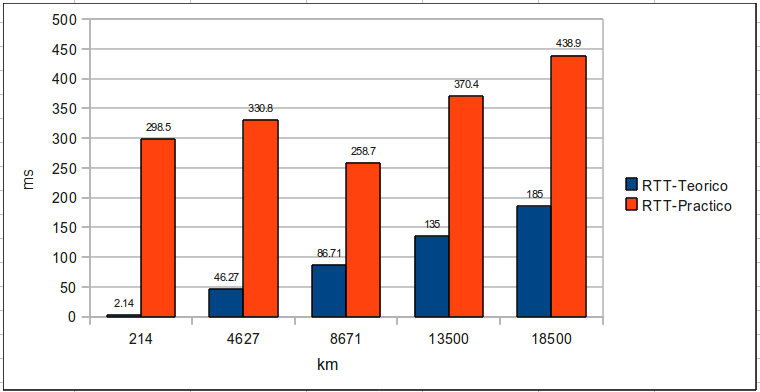
\includegraphics[scale=0.60]{graficos/comparacionRTT.png}
  \caption{Comparacion RTT teorico vs RTT practico }
\end{figure}


Lo que podemos observar en el gráfico es la gran diferencia entre el RTT teórico (calculado suponiendo un enlace punto a punto directo con el IP) y el práctico. Con estos podemos corroborar la existencia de un \textit{delay de red} muy elevado. Esto sucede por varias razones:
\begin{itemize}
	\item No existe enlace punto a punto con cada IP. El paquete enviado debe pasar por varios \textit{routers} antes de llegar al IP elegido.
	\item Cada \textit{router} agrega un delay correspondiente a la sobrecarga o congestión de la red en el momento en el que tiene que \textit{forwardear} el paquete. 
\end{itemize}

En el gráfico podemos notar algo que en un principio nos parecio \textit{raro}. El RTT práctico a EEUU, aunque la distancia es mayor que a Uruguay, es bastante menor. Esto se debe a que no contamos con un enlace directo a Uruguay, sino que el paquete da varios saltos para alcanzar el destino. No así con los EEUU, país con el cual tenemos un enlace más directo.  



\section{Segunda consigna}


\end{document}
